\begin{frame}
  \frametitle{\problemtitle}
  \begin{block}{Problem}
    Find the number of winning moves in a block stacking game:
    \begin{itemize}
      \item There are multiple stacks of blocks.
      \item Players alternate placing blocks on top of these.
      \item The first player unable to move loses.
      \item Each block must fit strictly within the one below it.
      \item There are three shapes with blocks of any integer size: circles, triangles, squares.
    \end{itemize} 
  \end{block}
  \vspace{5mm}
  \centering
  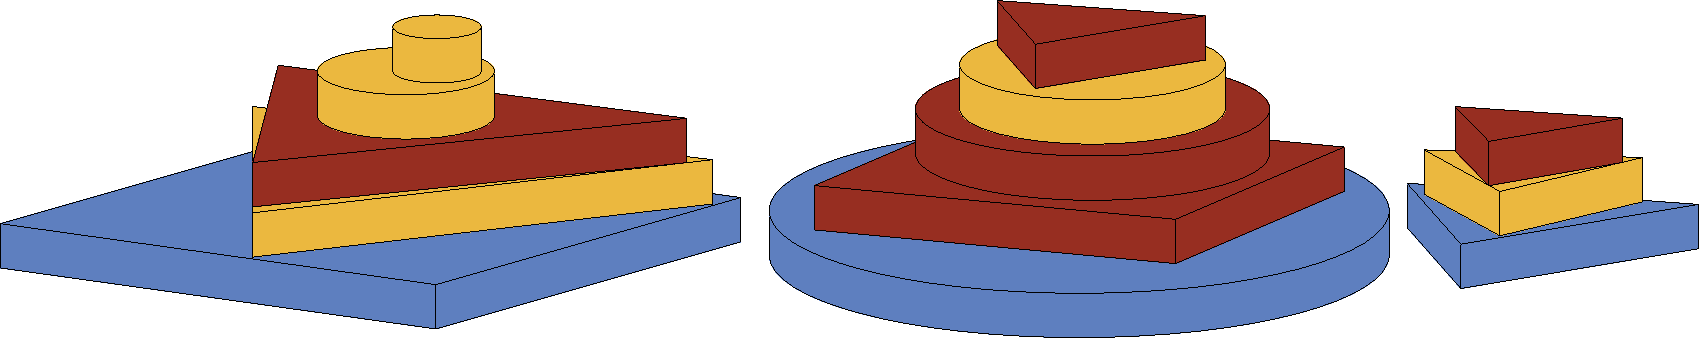
\includegraphics[width=0.8\textwidth]{image}
\end{frame}
\begin{frame}
  \frametitle{\problemtitle}
  \begin{block}{Subproblem}
    Given two blocks, determine if one of them fits inside the other.
  \end{block}
  \pause
  \begin{block}{Solution to Subproblem}
    \begin{itemize}
      \item<+-> Consider each pair of shapes ($\{\triangle,\Box,\bigcirc\}$) separately.
      \item<+-> For instance, if $\Box_m$ is a square with side length $m$ and $\bigcirc_n$ is a circle with radius $n$, then
        \[ \text{$\Box_m$ fits inside $\bigcirc_n$} \iff m < \sqrt{2}\cdot n. \]
      \item<+-> Similarly, for each $S,T\in\{\triangle,\Box,\bigcirc\}$, there exists some $\alpha_{S,T}$ such that
        \[ \text{$S_m$ fits inside $T_n$} \iff m < \alpha_{S,T}\cdot n. \]
      \item<+-> These numbers can be found using high school geometry. % such as the Pythagorean theorem and the law of cosines.
      \item<+-> \emph{Pitfall}: Near misses are possible, so use extended precision (\texttt{long double}, \texttt{BigDecimal}, \texttt{Decimal}).
    \end{itemize}
  \end{block}
\end{frame}
\begin{frame}
  \frametitle{\problemtitle}
  \begin{block}{Solution}
    \begin{itemize}
      \item<+-> This is a combinatorial game where for each stack we only care about its topmost block.
      \item<+-> Use the Sprague-Grundy theorem to assign each block $B$ a Grundy value $G(B)$.
      \item<+-> By careful analysis and/or dynamic programming we can find closed forms:
        \[
          G(\triangle_n) = n-1 \qquad
          G(\Box_n) = \lfloor(\sqrt{6}-\sqrt{2})n\rfloor \qquad
          G(\bigcirc_n) = \begin{cases}
            2, & \text{if $n=1$} \\
            \lfloor\sqrt{3}n\rfloor, & \text{otherwise}
          \end{cases}
        \]
      \item<+-> A position is losing iff the bitwise XOR of Grundy values of the stacks is $0$.
      \item<+-> For each stack, compute the Grundy value needed to create a losing position.
      \item<+-> For each shape, check whether a block with that Grundy value exists and constitutes a legal move.
      \item<+-> Total runtime: $\mathcal{O}(n)$.
    \end{itemize}
  \end{block}
\end{frame}
